\title{Supplemental material: High-dimensional estimation of mutual information via classification error}
\author{Charles Zheng and Yuval Benjamini}
\date{\today}

\documentclass[12pt]{article} 

% packages with special commands
\usepackage{amssymb, amsmath}
\usepackage{epsfig}
\usepackage{array}
\usepackage{ifthen}
\usepackage{color}
\usepackage{fancyhdr}
\usepackage{graphicx}
\usepackage{mathtools}
\usepackage{csquotes}
\definecolor{grey}{rgb}{0.5,0.5,0.5}

\begin{document}
\maketitle

\newcommand{\tr}{\text{tr}}
\newcommand{\E}{\textbf{E}}
\newcommand{\diag}{\text{diag}}
\newcommand{\argmax}{\text{argmax}}
\newcommand{\Cov}{\text{Cov}}
\newcommand{\Var}{\text{Var}}
\newcommand{\argmin}{\text{argmin}}
\newcommand{\Vol}{\text{Vol}}
\newcommand{\comm}[1]{}
\newcommand{\indep}{\rotatebox[origin=c]{90}{$\models$}}
\newcommand{\Cor}{\text{Cor}}

\section{Proofs}

\textbf{Lemma 1. }
\emph{
Suppose $(Z_1, Z_2, \hdots, Z_k)$ are jointly multivariate normal, with 
$\E[Z_1 - Z_i]= \alpha$, 
$\Var(Z_1) = \beta$, 
$\Cov(Z_1, Z_i) = \gamma$, 
$\Var(Z_i)= \delta$, and $\Cov(Z_i, Z_j) = \epsilon$ for all $i, j = 2, \hdots,
k$, such that $\beta + \epsilon - 2\gamma > 0$.  Then, letting
\[
\mu = \frac{\E[Z_1 - Z_i]}{\sqrt{\frac{1}{2}\Var(Z_i - Z_j)}} = \frac{\alpha}{\sqrt{\delta - \epsilon}},
\]
\[
\nu^2 = \frac{\Cov(Z_1 -Z_i, Z_1 - Z_j)}{\frac{1}{2}\Var(Z_i - Z_j)} = \frac{\beta + \epsilon - 2\gamma}{\delta - \epsilon},
\]
we have
\begin{align*}
\Pr[Z_1 < \max_{i=2}^k Z_i] &= \Pr[W < M_{k-1}]
\\&= 1 - \int \frac{1}{\sqrt{2\pi\nu^2}} e^{-\frac{(w-\mu)^2}{2\nu^2}} \Phi(w)^{k-1} dw,
\end{align*}
where $W \sim N(\mu, \nu^2)$ and $M_{k-1}$ is the maximum of $k-1$
independent standard normal variates, which are independent of $W$.
}

\textbf{Proof.}
We can construct independent normal variates $G_1$, $G_2,\hdots, G_k$
such that
\[
G_1 \sim N(0, \beta + \epsilon - 2 \gamma)
\]
\[
G_i \sim N(0, \delta - \epsilon)\text{ for }i > 1
\]
such that
\[
Z_1 - Z_i = \alpha + G_1 + G_i \text{ for }i > 1.
\]
Hence
\begin{align*}
\Pr[Z_1 < \max_{i=2}^k Z_i] &= \Pr[\min_{i > 1} Z_1 - Z_i < 0].
\\&= \Pr[\min_{i=2}^{k} G_1 + G_i + \alpha < 0]
\\&= \Pr[\min_{i=2}^{k} G_i < -\alpha - G_1]
\\&= \Pr[\min_{i=2}^{k} \frac{G_i}{\sqrt{\delta - \epsilon}} < -\frac{\alpha - G_1}{\sqrt{\delta - \epsilon}}].
\end{align*}
Since $\frac{G_i}{\sqrt{\delta - \epsilon}}$ are iid standard normal variates, and since
$-\frac{\alpha - G_1}{\sqrt{\delta - \epsilon}} \sim N(\mu,\nu^2)$ for $\mu$ and $\nu^2$ given in the statement of the Lemma, the proof is completed via a straightforward computation.  $\Box$

\textbf{Theorem 1.} Let $p^{[d]}(x, y)$ be a sequence of joint densities
for $d = 1,2,\hdots$ as given above.  Further assume that
\begin{itemize}
\item[A1.] $\lim_{d \to \infty} I(X^{[d]}; Y^{[d]}) = \iota < \infty.$
\item[A2.] There exists a sequence of scaling constants $a_{ij}^{[d]}$
and $b_{ij}^{[d]}$ such that the random vector $(a_{ij}\ell_{ij}^{[d]} +
b_{ij}^{[d]})_{i, j = 1,\hdots, k}$ converges in distribution to a
multivariate normal distribution.
\item[A3.] There exists a sequence of scaling constants $a^{[d]}$, $b^{[d]}$ such that
\[
a^{[d]}u(X^{(1)}, Y^{(2)}) + b^{[d]}
\]
converges in distribution to a univariate normal distribution.
\item[A4.] For all $i \neq k$,
\[\lim_{d \to \infty}\Cov[u(X^{(i)}, Y^{(j)}), u(X^{(k)}, Y^{(j)})] = 0.\]
\end{itemize}
Then for $e_{ABE, k}$ as defined above, we have
\[
\lim_{d \to \infty} e_{ABE, k} = \pi_k(\sqrt{2 \iota})
\]
where
\[
\pi_k(c) = 1 - \int_{\mathbb{R}} \phi(z - c)  \Phi(z)^{k-1} dz
\]
where $\phi$ and $\Phi$ are the standard normal density function and
cumulative distribution function, respectively.

%[[Maybe add remark about assumptions here.]]

\textbf{Proof.}

For $i = 2,\hdots, k$, define
\[
Z_i = \log p(Y^{(1)}|X^{(i)}) - \log p(Y^{(1)}|X^{(1)}).
\]
Then, we claim that $\vec{Z} = (Z_2,\hdots, Z_k)$ converges in distribution to
\[
\vec{Z} \sim N\left(-2\iota, 
\begin{bmatrix}
4\iota & 2\iota & \cdots & 2\iota\\
2\iota & 4\iota & \cdots & 2\iota\\
\vdots & \vdots & \ddots & \vdots\\
2\iota & 2\iota & \cdots & 4\iota
\end{bmatrix}
\right).
\]
Combining the claim with the lemma (stated below this proof) yields the
desired result.

To prove the claim, it suffices to derive the limiting moments
\[\E[Z_i] \to -2\iota,\]
\[\Var[Z_i] \to 4\iota,\]
\[\Cov[Z_i, Z_j] \to 2\iota,\]
for $i \neq j$,
since then assumption A2 implies the existence of a multivariate normal
limiting distribution with the given moments.

Before deriving the limiting moments, note the following identities.
Let $X' = X^{(2)}$ and $Y = Y^{(1)}$.
\[
\E[e^{u(X', Y)}] = \int p(x) p(y) e^{u(x, y)} dx dy = \int p(x, y) dx dy = 1.
\]
Therefore, from assumption A3 and the formula for gaussian exponential
moments, we have
\[
\lim_{d \to \infty} \E[u(X', Y)]-\frac{1}{2}\Var[u(X', Y)] = 0.
\]
Let $\sigma^2 = \lim_{d \to \infty} \Var[u(X', Y)]$.
Meanwhile, by applying assumption A2,
\begin{align*}
\lim_{d \to \infty} I(X; Y) &= \lim_{d \to \infty} \int p(x, y) u(x, y) dx dy 
= \lim_{d \to \infty} \int p(x) p(y) e^{u(x, y)} u(x, y) dx dy
\\&= \lim_{d \to \infty}  \E[e^{u(X, Y')}u(X, Y')]
\\&= \int_{\mathbb{R}} e^z z \frac{1}{\sqrt{2\pi \sigma^2}} 
e^{-\frac{(z + \sigma^2/2)^2}{2\sigma^2}} \text{ (applying A2)}
\\&= \int_{\mathbb{R}} z \frac{1}{\sqrt{2\pi \sigma^2}} 
e^{-\frac{(z - \sigma^2/2)^2}{2\sigma^2}}
\\&= \frac{1}{2}\sigma^2.
\end{align*}
Therefore,
\[
\sigma^2 = 2\iota,
\]
and
\[
\lim_{d \to \infty} \E[u(X', Y)] = -\iota.
\]
Once again by applying A2, we get
\begin{align*}
\lim_{d \to \infty} \Var[u(X, Y)] 
&= \lim_{d \to \infty} \int (u(x, y) - \iota)^2 p(x, y) dx dy
\\&= \lim_{d \to \infty} \int (u(x, y) - \iota)^2 e^{u(x, y)} p(x) p(y) dx dy
\\&= \lim_{d \to \infty} \E[(u(X', Y) - \iota)^2 e^{u(X', Y)}] 
\\&= \int (z - \iota)^2 e^z \frac{1}{\sqrt{4\pi\iota}} e^{-\frac{(z+\iota)^2}{4\iota}} dz \text{ (applying A2)}
\\&= \int (z - \iota)^2 \frac{1}{\sqrt{4\pi\iota}} e^{-\frac{(z-\iota)^2}{4\iota}} dz
\\&= 2\iota.
\end{align*}


We now proceed to derive the limiting moments.
We have
\begin{align*}
\lim_{d \to \infty} \E[Z] 
&= \lim_{d \to \infty} \E[ \log p(Y|X') - \log p(Y|X)]
\\&= \lim_{d \to \infty} \E[ u(X', Y) - u(X, Y) ] = -2\iota.
\end{align*}
Also,
\begin{align*}
\lim_{d \to \infty} \Var[Z]
 &= \lim_{d \to \infty} \Var[ u(X', Y) - u(X, Y) ]
\\&= \lim_{d \to \infty} \Var[ u(X', Y)] +\Var[ u(X, Y) ]\text{ (using assumption A4) }
\\&= 4\iota,
\end{align*}
and similarly
\begin{align*}
\lim_{d \to \infty} \Cov[Z_i, Z_j]
&= \lim_{d \to \infty} \Var[ u(X, Y)]\text{ (using assumption A4) }
\\&= 2\iota.
\end{align*}
This concludes the proof. $\Box$.

\subsection{Assumptions of theorem 1}

Assumptions A1-A4 are satisfied in a variety of natural models.
One example is a multivariate Gaussian model where
\[
X \sim N(0, \Sigma_d)
\]
\[
E \sim N(0, \Sigma_e)
\]
\[
Y = X + E
\]
where $\Sigma_d$ and $\Sigma_e$ are $d \times d$ covariance matrices, and where $X$ and $E$ are independent.  Then, if $d \Sigma_d$ and $\Sigma_e$ have limiting spectra $H$ and $G$ respectively,
the joint densities $p(x, y)$ for $d = 1,\hdots, $ satisfy assumptions A1 - A4.

We can also construct a family of densities satisfying A1 - A4,
which we call an \emph{exponential family sequence model} since each joint distribution in the sequence
is a member of an exponential family.
A given exponential family sequence model is specified by choice of a base carrier function $b(x, y)$ and base sufficient statistic $t(x, y)$, with the property that carrier function factorizes as
\[
b(x, y) = b_x(x) b_y(y)
\]
for marginal densities $b_x$ and $b_y$.
Note that the dimensions of $x$ and $y$ in the base carrier function are arbitrary;
let $p$ denote the dimension of $x$ and $q$ the dimension of $y$ for the base carrier function.
Next, one specifies a sequence of scalar parameters $\kappa_1, \kappa_2,\hdots$ such that
\[
\lim_{d \to \infty} d \kappa_d = c < \infty.
\]
for some constant $c$.
For the $d$th element of the sequence, $X^{[d]}$ is a $pd$-dimensional vector,
which can be partitioned into blocks
\[
X^{[d]} = (X_1^{[d]},\hdots, X_d^{[d]})
\]
where each $X_i^{[d]}$ is $p$-dimensional.  Similarly, $Y^{[d]}$ is partitioned into $Y_i^{[d]}$ for $i = 1,\hdots, d$.
The density of $(X^{[d]}, Y^{[d]})$ is given by
\[
p^{[d]}(x^{[d]}, y^{[d]}) = Z_d^{-1} \left(\prod_{i=1}^d b(x_i^{[d]}, y_i^{[d]}) \right) 
\exp\left[\kappa_d \sum_{i=1}^d t(x_i^{[d]}, y_i^{[d]}) \right],
\]
where $Z_d$ is a normalizing constant.
Hence $p^{[d]}$ can be recognized as the member of an exponential family with carrier measure
\[
\left(\prod_{i=1}^d b(x_i^{[d]}, y_i^{[d]}) \right)
\]
and sufficient statistic
\[
\sum_{i=1}^d t(x_i^{[d]}, y_i^{[d]}).
\]

One example of such an exponential family sequence model is a
multivariate Gaussian model with limiting spectra $H = \delta_1$ and
$G = \delta_1$, but scaled so that the marginal variance of the
components of $X$ and $Y$ are equal to one.  This corresponds to a
exponential family sequence model with
\[
b_x(x) = b_y(x) = \frac{1}{\sqrt{2\pi}} e^{-x^2/2}
\]
and
\[t(x, y) = xy.\]

Another example is a multivariate logistic regression model,
given by
\[
X \sim N(0, I)
\]
\[
Y_i \sim \text{Bernoulli}(e^{\beta X_i}/(1 + e^{\beta X_i}))
\]
This corresponds to an exponential family sequence model with
\[
b_x(x) = \frac{1}{\sqrt{2\pi}} e^{-x^2/2}
\]
\[
b_y(y) = \frac{1}{2}\text{ for }y = \{0, 1\},
\]
and
\[
t(x, y) = x\delta_1(y) - x\delta_0(y).
\]
The multivariate logistic regression model (and multivariate Poisson regression model)
are especially suitable for modeling neural spike count data;
we simulate data from such a multivariate logistic regression model in section X.

\section{Additional simulation results}

Multiple-response logistic regression model
\[
X \sim N(0, I_p)
\]
\[
Y \in \{0,1\}^q
\]
\[
Y_i|X = x \sim \text{Bernoulli}(x^T B_i)
\]
where $B$ is a $p \times q$ matrix.

\emph{Methods.}
\begin{itemize}
\item \text{Nonparametric}: $\hat{I}_0$ naive estimator, $\hat{I}_\alpha$ anthropic correction.
\item \text{ML-based}: $\hat{I}_{CM}$ confusion matrix, $\hat{I}_F$ Fano, $\hat{I}_{HD}$ high-dimensional method.
\end{itemize}

Sampling distribution of $\hat{I}$ for \small{$\{p = 3$, $B
= \frac{4}{\sqrt{3}} I_3$, $K = 20$, $r = 40\}$.}

True parameter $I(X; Y) = 0.800$ \emph{(dotted line.)}
\begin{center}
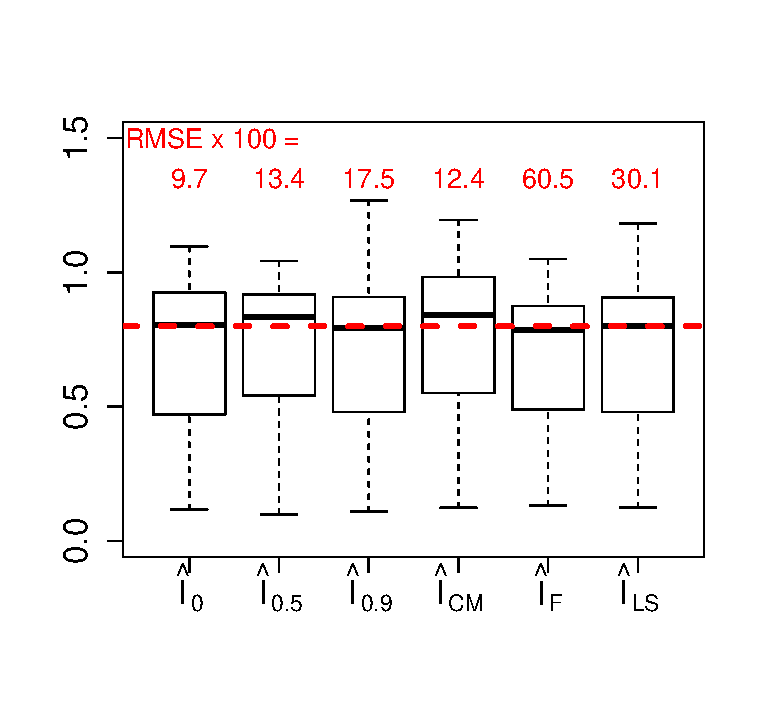
\includegraphics[scale = 0.5, clip = true, trim = 0 0.5in 0 0.5in]{../info_theory_sims/fig1.pdf}
\end{center}
Na\"{i}ve estimator performs best!  $\hat{I}_{HD}$ not effective.

Sampling distribution of $\hat{I}$ for \small{$\{p = 50$, $B = \frac{4}{\sqrt{50}} I_{50}$, $K = 20$, $r = 8000\}$.}

True parameter $I(X; Y) = 1.794$ \emph{(dashed line.)}
\begin{center}
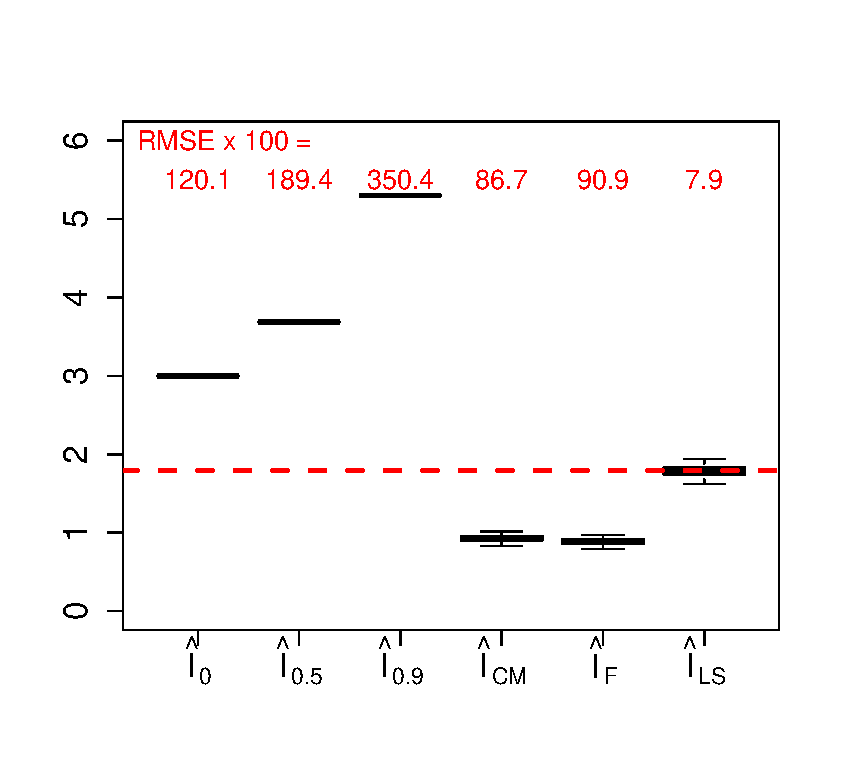
\includegraphics[scale = 0.5, clip = true, trim = 0 0.5in 0 0.5in]{../info_theory_sims/fig2.pdf}
\end{center}
Non-parametric methods extremely biased.

Estimation path of $\hat{I}_{HD}$ and $\hat{I}_\alpha$ as $n$ ranges from $10$ to $8000$.

\small{$\{p = 10$, $B = \frac{4}{\sqrt{10}} I_{10}$, $K = 20\}$.
True parameter $I(X; Y) = 1.322$ \emph{(dashed line.)}}

\begin{center}
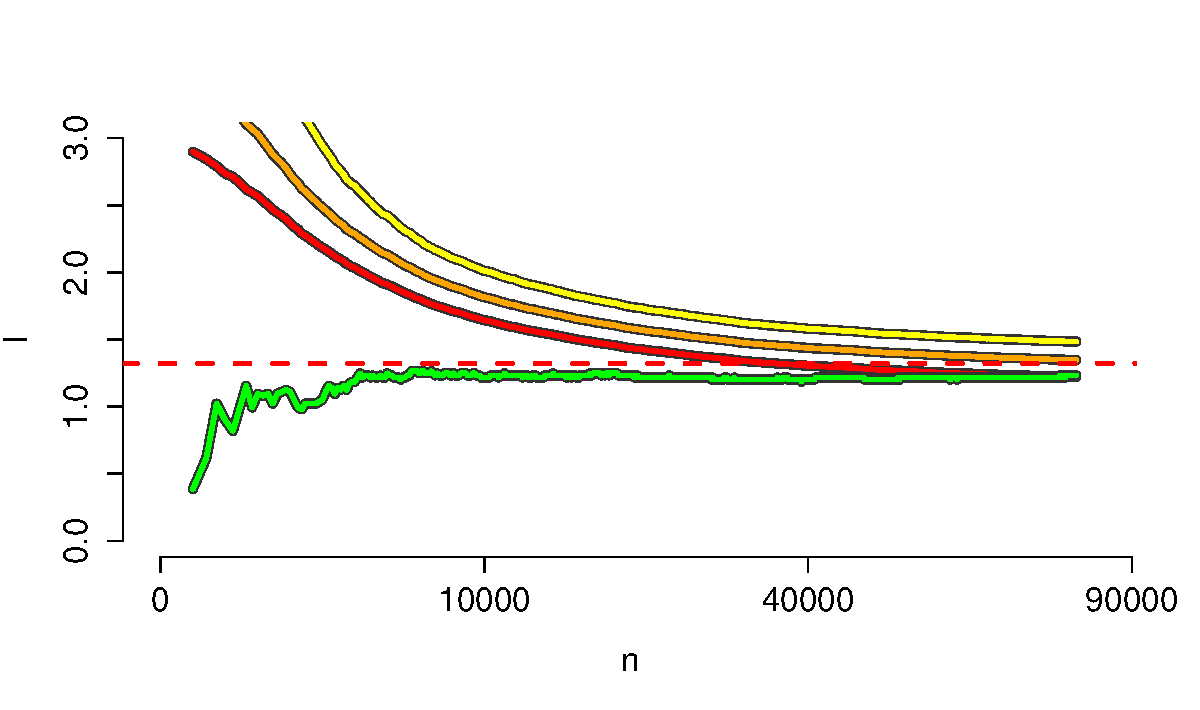
\includegraphics[scale = 0.4]{../info_theory_sims/fig3.pdf}
\end{center}

\begin{center}
\textbf{Estimated $\hat{I}$ vs true $I$.} 

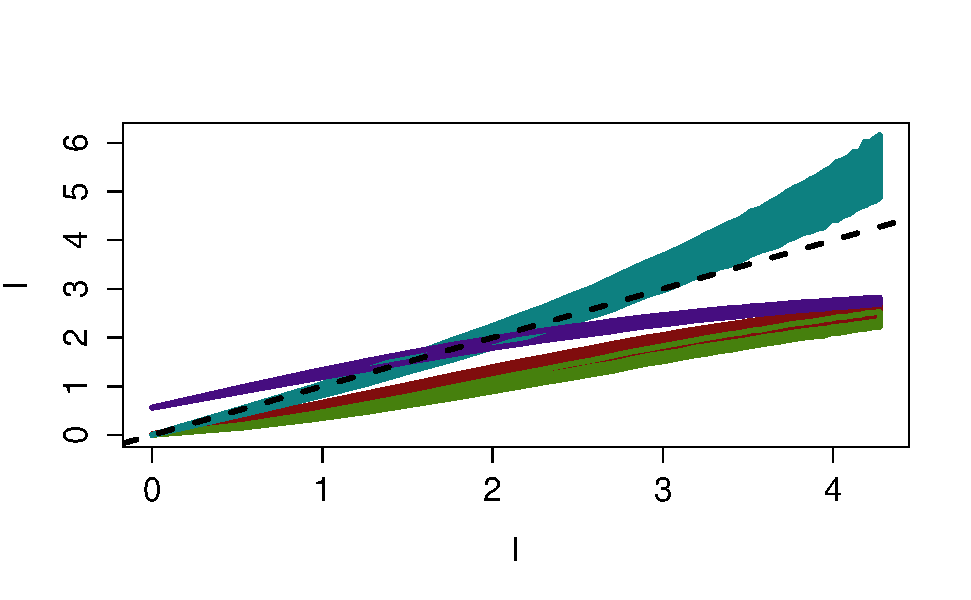
\includegraphics[scale = 0.5, clip=true, trim=0.4in 0.5in 0 0.5in]{../info_theory_sims/fig4.pdf}
\end{center}

Sampling distribution of $\hat{I}_{HD}$ for \small{$\{p = 10$, $B = \frac{4}{\sqrt{10}} I_{10}$, $N = 80000\}$,

and $K = \{5, 10, 15, 20, \hdots, 80\}$, $r = N/k$.}

True parameter $I(X; Y) = 1.322$ \emph{(dashed line.)}
\begin{center}
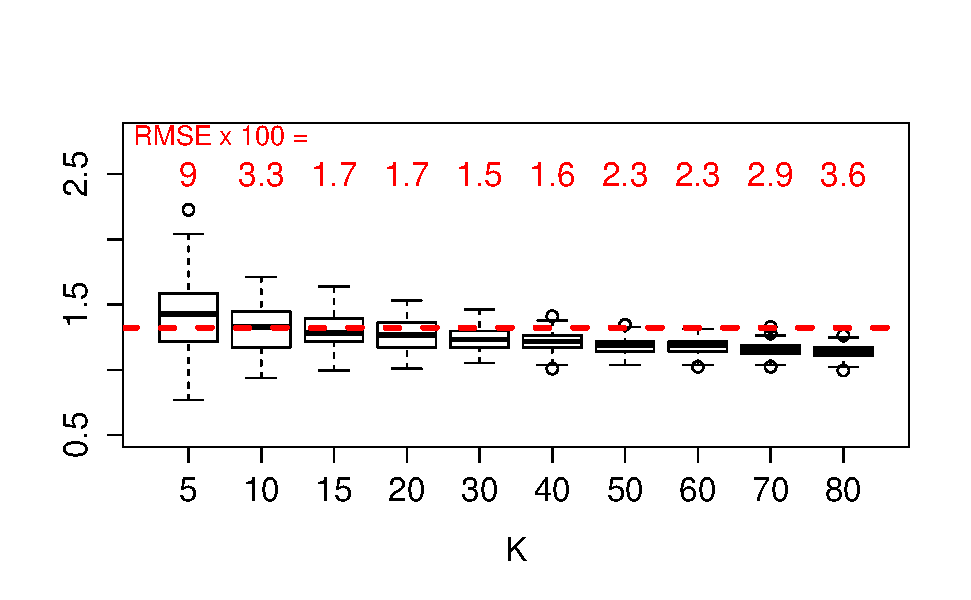
\includegraphics[scale = 0.6, clip = true, trim = 0 0.5in 0 0.5in]{../info_theory_sims/fig5a.pdf}
\end{center}

Decreasing variance as $K$ increases. Bias at large and small $K$.

$p = 20$ and $q = 40$, entries of $B$ are iid $N(0, 0.025)$.

$K=20$, $r = 8000$, true $I(X; Y) = 1.86$ \emph{(dashed line.)}

\begin{center}
\textbf{Sampling distribution of $\hat{I}$.}
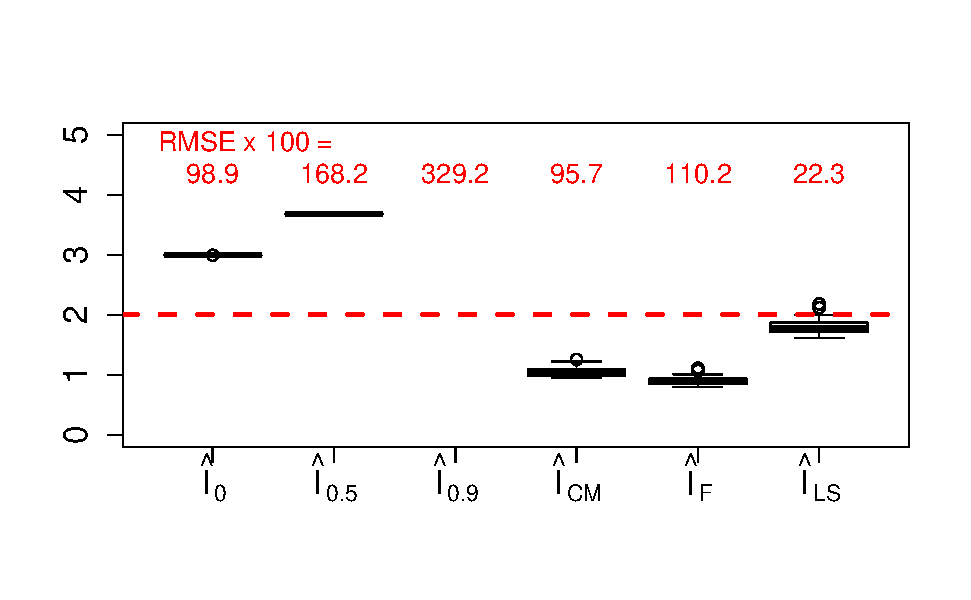
\includegraphics[scale = 0.6, clip = true, trim = 0 0.5in 0 0.5in]{../info_theory_sims/fig6.pdf}
\end{center}

\section{References}
\begin{itemize}
\item Cover and Thomas.  Elements of information theory.
\item Muirhead.  Aspects of multivariate statistical theory.
\item van der Vaart.  Asymptotic statistics.
\end{itemize}
\end{document}





